\documentclass[a4paper, 12pt, oneside]{book}
\usepackage{microtype} %used to manage hyphenations
\usepackage[utf8]{inputenc}% for the accents
\usepackage[T1]{fontenc}
\usepackage{mathptmx}
\usepackage{graphicx}
\usepackage{afterpage}
\usepackage{mathtools}
\usepackage{amsmath}
\usepackage{amsfonts}
\usepackage{xspace}
\usepackage{float} %to control the floating environments
\usepackage[a4paper, inner=2.54cm, outer=2.54cm, top=2.54cm, bottom=2.54cm, bindingoffset=1cm]{geometry}
\frenchspacing
\renewcommand{\bibname}{References}
\setcounter{tocdepth}{3}

%temporary packages
\usepackage[english]{babel}
\usepackage{blindtext}
% \usepackage{titlesec}
%
% \titleclass{\chapter}{straight}
%using one half spacing between lines.
\usepackage[onehalfspacing]{setspace}

\usepackage{paralist}
\usepackage{hyperref}
\usepackage{cleveref}

\usepackage{array}
\usepackage{booktabs}


\newcommand{\head}[1]{\textbf{#1}}
\newcommand{\yhat}{\hat{y}}
\setlength{\abovetopsep}{10pt}
\DeclareUnicodeCharacter{2212}{-}

\begin{document}
\frontmatter
%the entire document will be divided into chapters only.
\chapter*{Abstract}
\blindtext
\addcontentsline{toc}{chapter}{Abstract}
\nopagebreak

\chapter*{Acknowledgement}
\blindtext
\addcontentsline{toc}{chapter}{Acknowledgement}

\tableofcontents
\addcontentsline{toc}{chapter}{\contentsname}
\listoftables
\addcontentsline{toc}{chapter}{\listtablename}
\listoffigures
\addcontentsline{toc}{chapter}{\listfigurename}
\addtocontents{toc}{\bigskip}

\chapter{List of Abbreviations}

\begin{description}

  \item[CNN] Convolutional neural networks
  \item[ANN] Artifitial neural networks

\end{description}

\mainmatter

\chapter*{Introduction}
\addcontentsline{toc}{chapter}{Introduction}
\blindtext[5]

\chapter{Feed-Forward neural networks}
To understand the technique used in this report, it is necessary to understand basic neural networks functioning.
Given a scenario with a training set of labeled data $(\textbf{x}, \textbf{y})$, where $\textbf{x}$ denotes the training example
composed of multiple features, say $\textbf{x} = \{x_{1}, x_{2}, \ldots, x_{n}\}$, and \textbf{y} the corresponding label.
Let's introduce the idea of `perceptron'. \\
Perceptrons are the building blocks of neural networks, and the best way to get stated is with an example.
Assume at the university's admission office the students are evaluated with two pieces of information, the results of a test and their grades in school. Let's take a look at some sample students, see \cref{fig:perceptron}.

\begin{figure}[ht]
  \centering
  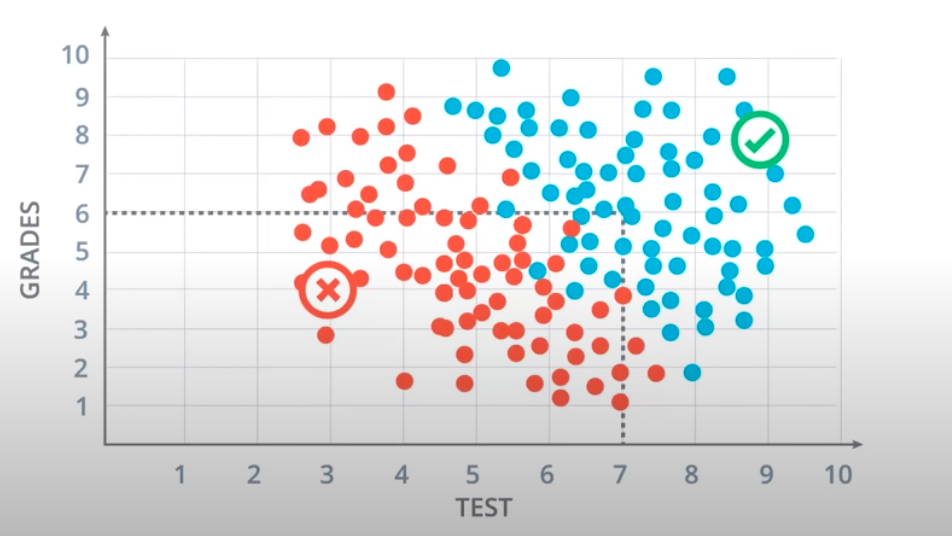
\includegraphics[width=0.7\textwidth]{figs/fig1.png}
  \caption{test vs grades }\label{fig:perceptron}
\end{figure}

The data on the figure can be nicely separated with a line, where most students above the line get accepted and most students under the line get rejected, see \cref{fig:line}. Therefore this line is going to be our model. \\
The model makes a couple of mistakes since there are a few blue points that are under the line and few over the line, but they are considered as noise and add no new information to our model. Now, the natural question that arises: how do we find the line ?

\begin{figure}[htbp]
  \centering
  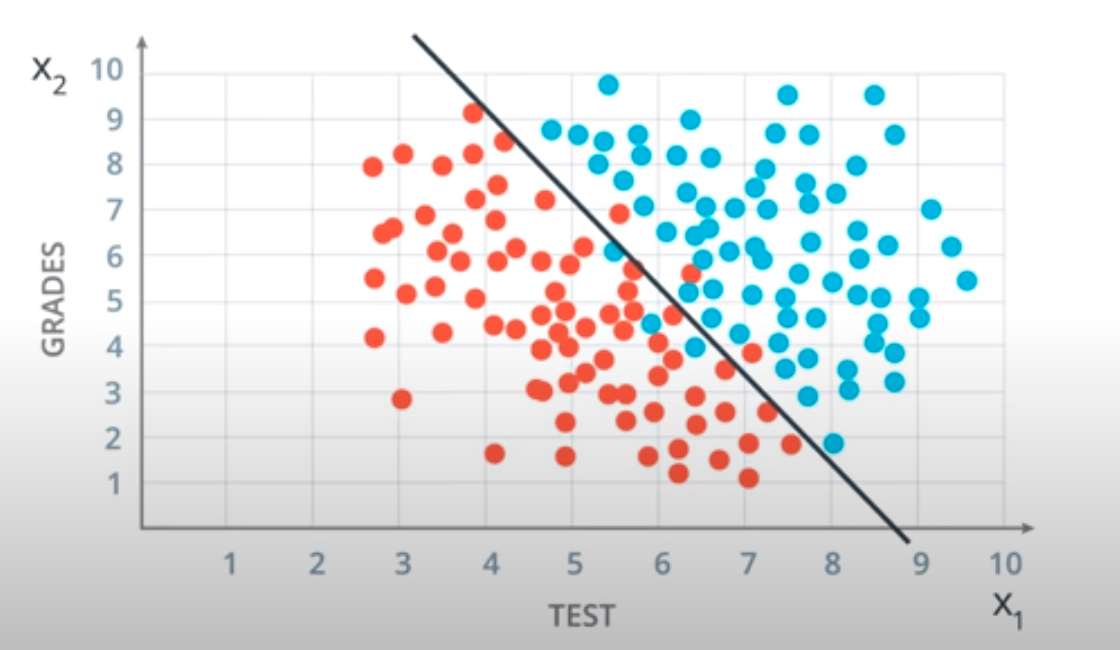
\includegraphics[width=0.7\textwidth]{figs/fig2.png}
  \caption{seperating line}\label{fig:line}
\end{figure}

We start by labeling the axis $\textbf{x} = \{x_{1}, x_{2}\}$.
The boundary line separating the students has a linear equation
specifically: $2x_{1} + x_{2} - 18 = 0$.
Plotting the grades in the equation gives rise to a score, if the score is positive --the student
gets plotted in above the line--, the student gets accepted with otherwise not. This is called a prediction.\\

In a more general case, our boundary will be an equation of the following form:

$$w_{1}x_{1} + w_{2}x_{2} + b = 0.$$

Abbreviating this equation into vector notation:

\begin{equation}
  \label{linear}
  \textbf{w}\cdot\textbf{x} + b = 0
\end{equation}

Where $\textbf{w} = \{w_{1}, w_{2}\}$. We refer to $\textbf{x}$ as the input, $\textbf{w}$ as the weights and $b$ as the bias. Here $\textbf{y} = \{0, 1\}$ is the label, where 0 indicates the student being rejected whereas 1 indicates the student being accepted. Finally, our prediction is going to be called \mbox{\boldmath{$\hat{y}$}} and it will be what the algorithm predicts that the label will be, namely:

\begin{equation}
  \label{y_hat}
  \hat{y} =
  \begin{dcases*}
    \text{1,}  &$w\cdot x + b \geq 0$ \\
    \text{0,}  &$w\cdot x + b < 0$
  \end{dcases*}
\end{equation}

and the goal of the algorithm is to have \mbox{\boldmath{$\hat{y}$}} resembling \mbox{\boldmath{$y$}} as closely as possible. Reorganizing the equations in a graph and generalizing, gives rise to \cref{fig:neuron}. Here the bias is consider as a dummy input with value 1 to the Perceptron with weight b.

% \afterpage{\cleardoublepage}
\begin{figure}[H]
  \centering
  \includegraphics[width=0.7\textwidth]{figs/perceptron.png}
  \caption{perceptron's graph representation}\label{fig:neuron}
\end{figure}

% \section{activation functions}
%
% Giving a training set, the classification of the input vector is based upon $\textbf{w}$, therefore the goal of the algorithm is to determine those
% weights through an iterative process. The probelm given here is that the algorithm can only learn linear functions since the output of the perceptron
% is a simple linear combination of the input. In real world situation, the data is much more complex and highly non-linear, therefore to remedy this
% problem we shall introduce a non-linearty in our algorithm, called \textbf{activation function} in deep learning literature. Namely the sigmoid
% function.
%
% $$
% \sigma(x) = \frac{1}{1 + e^{-x}}
% $$
%
% One important property of an activation function is differentiability, because as we are going to explore in section, gradient descent will be used as optimizer to determine the networks' weights, in contrast to the perceptron which uses a discrete activation. That sigmoid function can be seen as continuous version of the perceptron's discrete activation function. Indeed:
%
%
%
%
% Instead of returning 0 or 1, the sigmoid function returns the probability of an event occuring, thus in our example the sigmoid function would output
% the probability of a student getting accepted or rejected, which can be expressed as the the conditional probability $p(y=1 | x) = \sigma(w\cdot x +
% b)$. There several other activation functions that can be used depending on the problem at hand. For example if a neural network is used to predict
% continuous non-bounded function that takes values in the interval $]-\infty, +\infty[$, then a more clever choice is the linear activation
% funciton, which is defined as: $f(x) = x$.


\section{Cost function}\label{cost}

In order to estimate the accuracy of the algorithm, or otherwise stated determine how well a certain prediction given by the algorithm is, we may establish a cost function, which measures the error the algorithm makes on some prediction (cost function is often referred to as error function). There are more that one choice for such a function. \Cref{equ:mse} can be used, it is called ``The Mean Squared Error''.

\begin{equation}
  \label{equ:mse}
  L(w, b) = \frac{1}{2} \sum_{i = 1}^{n} ||y - \hat{y}||^2.
\end{equation}

This function, becomes large when our network approximates $y$ badly, and small when the approximation is accurate. Additionally notice that if we set $L_x = \frac{1}{2} (y - \hat{y})^2$ we have that:
\begin{equation}
  \label{equ:additivity}
  L(w,b) = \sum_{i = 1}^{n} L_{x_{i}}.
\end{equation}
This property will be important in the algorithm described in Section 2.2.3.

Another way of defining a cost function is using the ``The Maximum Likelihood Estimation'' technique, since the sigmoid function deals with probabilities. We take the joint probability of the entire training set, assuming the training examples being independent events:

\begin{equation}
  \label{equ:likelihood}
  L(w, b) = p(y^{(1)}, y^{(2)}, \ldots, y^{(n)} | x^{(1)}, \ldots, x^{(n)}) = \prod_{i=1}^{n} p(y^{(i)}|x^{(i)})
\end{equation}

where $x^{(i)}$, $y^{(i)}$ represent the $i^{th}$ training example and label respectively. Thus by maximizing the joint probability, or respectively minimizing the $-\log$ of the likelihood, we can get an estimate of the parameters $w \ and \ b $. Now, in our worked example, the neural network can be treated as a random variable having a Bernoulli distribution, therefore \cref{equ:likelihood} can be rewritten as follows:

\begin{equation}
  \label{equ:b_likelihood}
  L(w, b) = - \sum_{i = 1}^{n} y_i \log(\hat{y}) + (1 - y) \log(1 - \hat{y}).
\end{equation}

\Cref{equ:b_likelihood} is usually the cost function used for Bernoulli distributed labeled data. It is often referred to as \textbf{binary cross-entropy} or BCE for short.

For multi-class classification (predicting multiple classes, say $k$ classes), a similar idea can used considering a multinoulli distribution on the data set where $p(y | \textbf{x}) = \prod_{i = 1}^{k} p_i^{[y=i]}$, where $[y = i]$ evaluates to 1 if $x = i$, 0 otherwise. This leads to following cost function using MLE

\begin{equation}
  \label{equ:m_likelihood}
  L(w, b) = - \sum_{j = 1}^k \sum_{i = 1}^{n} y_{i, j} \log(\hat{y}_{i, j}).
\end{equation}

\section{Gradient descent}
In order to minimize the cost function we rely on optimization algorithms from numerical methods as it is unpractical to solve manually. The technique used in deep learning is the gradient descent. \\
The gradient of a differentiable function $f: \mathbb{R}^n \longrightarrow \mathbb{R}$ at a point $x = (x_1, \ldots, x_n) \in \mathbb{R}^n$ is a vector in $\mathbb{R}^n$ of the form

\begin{equation}
  \label{equ:gradient}
  \nabla f(x) = (\frac{\partial f}{\partial x_1} (x), \ldots, \frac{\partial f}{\partial x_n} (x))
\end{equation}

It is a well known result that, given a point $x \in \mathbb{R}^n$, the gradient at that point the direction of steepest ascent. Given that $f$ is differentiable at $x$, the vector $-\nabla f(x)$ indicates the direction of steepest descent of the function $f$ at the point $x$.
In order to obtain the minimum value of the function, the gradient descent strategy tells us to start at a given $x_0 \in \mathbb{R}^n$, calculate the value of $\nabla f(x_0)$, and then proceed to calculate a new point $x_1 = x_0 − \alpha \nabla f(x_0)$, where $\alpha > 0$ is called the \textbf{learning rate}. We then repeat this process, creating a sequence $\{ x_i \}$ defined by our initial choice of $x_0$, the learning rate $\alpha$, and the rule: $x_{i + 1} = x_{i} − \alpha \nabla f(x_0)$  . This sequence continues until we approach a region close to our desired minimum.
The method of gradient descent when taken continuously over infinitesimally small increments (that is, taking the limit $\alpha \rightarrow 0$) usually converges to a local minimum. However, depending on the location of the initial $x_0$, the local minimum achieved may not be the global minimum of the function. Furthermore, since when carrying out calculations on an unknown function we must take discrete steps (which vary in length depending on the learning rate), we are not even guaranteed a local minimum but rather may oscillate close to one, or even ’jump’ past it altogether if the learning rate is too big. Still, even with these possible complications, gradient descent is a surprisingly successful method for many real life applications and is the most standard method of training for feed-forward neural networks and many other machine learning algorithms.
Given that our cost function indicates how poorly our neural network approximates a given function, by calculating the gradient of the cost function with respect to the weights and biases of the network and adjusting these parameters in the direction opposite to the gradient, we will decrease our error and therefore lead us closer to an adequate network (in most cases) see .

\subsection{Gradient calculation}\label{sec:cal_gradient}

Before applying the gradient descent technique, we can clearly see that the an output of 0 or 1 is problematic since the derivatives would be 0. Therefore the gradient descent technique will not work. To remedy this, following the MLE, a Bernoulli distribution has been defined on $y$, therefore the neural net needs to predict $\yhat = p(y = 1 | x) = \sigma (x)$. For this number to be a valid probability, it must lie in the interval $[0, 1]$. \\
A good approach would ensure the existence of a strong gradient whenever the model has the wrong answer. And for consistency with the perceptron's decision rule (\cref{y_hat}), a very positive linear combination of the input $x$ has to have a probability close to 1 and vise versa (see \cref{fig:step_sigmoid}), otherwise

\begin{equation}
  \label{equ:limits}
  \lim_{x \rightarrow +\infty} \sigma(x) = 1, \qquad \lim_{x \rightarrow -\infty} \sigma(x) = 0.
\end{equation}

This approach is based on the sigmoid function:
 $$
 \sigma(x) = \frac{1}{1 + e^{-x}}
 $$

This function is suitable for the problem at hand, namely binary classification. However, depending on the output $\yhat$ other functions might be used. For example if a neural network is used to predict continuous non-bounded function that takes values in the interval $]-\infty, +\infty[$, then a more clever choice is the linear activation function, which is defined as: $f(x) = x$. Another example is the multi-class classification, where a multinoulli distribution is defined over the training data. The function used is the softmax defined as

$$
softmax(x_i) = \frac{e^{x_i}}{\sum_j e^{x_j}}
$$

Where $x_i$ represents a training example from class $i$. Here the output consists of $j$ outputs rather that a single one. See \cref{fig:ann} to illustrate the output layer.

\begin{figure}[!htpb]
  \centering
  \includegraphics[width=\textwidth]{figs/step_sigmoid.png}
  \caption[sigmoid vs step function]{sigmoid vs step function. The two plots clearly show cast the continuity of the sigmoid.}\label{fig:step_sigmoid}
\end{figure}

Now, let us apply the gradient descent technique to our network. Our goal is to calculate the gradient of $L$ at a point $x = (x_1, \ldots, x_n)$ given by the partial derivatives, see \cref{equ:gradient}. In addition, the property \cref{equ:additivity} now become important. In fact, we are only going to calculate the value of $\nabla L_x$ for a given labeled data point and then add the values of the gradient together, see below.

\begin{equation}
  \nabla L(w, b) = \nabla (\sum_{i = 1}^{n} L_x) = \sum_{i = 1}^{n} \nabla L_{x_i}.
\end{equation}

The error produced by each point is simply: $ L_x = -y \log (\hat{y}) - (1 - y) \log (1 - \hat{y})$. In order to calculate the derivative of this error with respect to the weights, we'll first calculate $ \frac{\partial}{\partial w_j} \hat{y}$, where $ \hat{y} = \sigma (w \cdot x + b)$.

\begin{align*}
  \frac{\partial}{\partial w_j} \hat{y} &= \frac{\partial}{\partial w_j} \sigma (w \cdot x + b) \\
     &= \sigma (w \cdot x + b) (1 - \sigma (w \cdot x + b)) \cdot \frac{\partial}{\partial w_j} (w \cdot x + b) \\
     &= \hat{y} (1 - \hat{y}) \cdot \frac{\partial}{\partial w_j} (w \cdot x + b) \\
     &= \hat{y} (1 - \hat{y}) \cdot \frac{\partial}{\partial w_j} (w_1 x_1 + \ldots + w_j x_j + \ldots w_n x_n + b) \\
     &= \hat{y} (1 - \hat{y}) \cdot x_j.
\end{align*}

Now we can go ahead and calculate the derivative of the error $L$ at a point $x$, with respect to the weight $w_j$.

\begin{align*}
  \frac{\partial}{\partial w_j} L_x &= \frac{\partial}{\partial w_j} [-y \log (\hat{y}) - (1 - y) \log (1 - \hat{y})] \\
     &= -y \frac{\partial}{\partial w_j} \log (\yhat) - (1 - y) \frac{\partial}{\partial w_j} (1 - \yhat) \\
     &= -y \frac{1}{\yhat} \cdot \frac{\partial}{\partial w_j} \yhat - (1 - y) \frac{1}{1 - \yhat} \cdot \frac{\partial}{\partial w_j} (1 - \yhat) \\
     &= -y (1 - \yhat) \cdot x_j + (1 - y)\yhat \cdot x_j \\
     &= -(y - \yhat) x_j
\end{align*}

A similar calculation will show that

$$
\frac{\partial}{\partial b} L_x = -(y - \yhat)
$$

Therefore, since the gradient descent step simply consists in subtracting a multiple of the gradient of the error function at every point, then this updates the weights in the following way:

\begin{align}
  w^{\prime}_i &= w_i + \alpha (y - \yhat)x_i \\
  b^{\prime} &= b + \alpha (y - \yhat)
\end{align}

\section{Neural network architecture}
In our work example, the target function was a simple linear function. However, in real world situations the input data is much more complex and often cannot be separated with a line. That is where neural nets shine. Neural networks also referred to as \textbf{feedforward} neural nets or \textbf{multilayer perceptron} (MLPs) are as the name indicates are stacks of perceptrons, where each \textbf{unit} receives the input $x$, calculates the inner product with a set of weights and apply a non-linearity to the result, then these results are fed to a next layer of units that does the same calculations and so on. The overall length of the chain gives the \textbf{depth} of the model. The final layer of such a network is called the \textbf{the output layer}, whereas the intermediate layer are referred to as \textbf{hidden layers}. The goal of the feed-forward network is to approximate some function $f^*$. The training example specify directly what the output layer must do at each point $x$; it must produce a value that is close to $y$. Therefore, the function computed after the linear combination is important. This function and the functions used in the hidden layers are referred to as \textbf{activation functions}. For example for a classifier, the function maps an input $x$ to a category $y$, a natural choice of activation is the sigmoid; whereas in a regression problem, where the output is continuous non-bounded that takes values in the interval $]-\infty, +\infty[$, a more clever choice is the linear activation function, which is defined as: $f(x) = x$.
The figure below depicts the architecture described above.

\begin{figure}[!htpb]
  \centering
  \includegraphics[width=\textwidth]{figs/nn.png}
  \caption[A visual representation of a feed-forward network]{A visual representation of a feed-forward network which approximates some function $f : \mathbb{R}^n \longrightarrow \mathbb{R}^m$ by
    computing the function $f^*(x) = (f^*_1(x), \ldots, f^*_m(x))$. In this approach, the network is shown as a
    directed weighted graph. Here $x = (x_1, \ldots, x_n)$}\label{fig:ann}
\end{figure}

For notation, set $w^n_{a, b} \in \mathbb{R}$ as the weight between the $a^th$ unit in the $(n - 1)^th$ layer with $k$ units to the $b^th$ unit in the $n^th$ layer with $j$ units.

\begin{equation}
  w_n = \begin{pmatrix}
    w^n_{1, 1} & \ldots & w^n_{1, k} \\
    \vdots & \ddots & \vdots \\
    w^n_{j, 1} & \ldots & w^n_{j, k}
  \end{pmatrix}
\end{equation}

The bias can be added as a dummy unit with input $x_{n+1} = 1$, which is a constant $b \in \mathbb{R}^j$. In order to calculate the output $a_n$ of the $n^th$ layer, we use the formula

$$
a_n = \sigma (w_n \cdot a_{n - 1} + b_n).
$$

In the above equation, the activation function $\sigma$ is applied element-wise to each element of the resulting vector. As the computations are carried out along the network's layers, the final function $f$ calculated by a network of depth $N$ is

$$
f(x) = \sigma(w_N\sigma(\ldots\sigma (w_2 \sigma(w_1 \cdot x + b_1) + b_2)) + b_N)
$$

\section{Back-propagation}
In order to train a neural network, the same techniques are used as in \cref{sec:cal_gradient}. First we define a cost function (which is the same as in the perceptron algorithm \cref{equ:b_likelihood},but with a much more complex $\yhat$), we calculate the feed-forward pass (we calculate the output $\yhat$), and then calculate the the gradient of the cost function $L$ with respect to every single weight and bias in the network, we get the following gradient vector $\nabla L = (\ldots, \frac{\partial}{\partial w^l_{i, j}} L, \ldots)$. Then applying the gradient step look likes

\begin{align*}
  w^{\prime l}_{i, j} &= w^l_{i, j} - \alpha  \frac{\partial}{\partial w^l_{i, j}} L\\
  b^{\prime l}_j &= b_j - \alpha \frac{\partial}{\partial b^l_j} L
\end{align*}

The big challenge of applying gradient descent to neural networks is calculating these partial derivatives.  This is where back-propagation comes in. This algorithm first tells us how to calculate these values for the last layer of connections, and with these results then inductively goes "backwards" through the network, calculating the partial derivatives of each layer until it reaches the first layer of the network. Hence the name "back-propagation".

For the purpose of this section it is useful to consider the values of each layer before the activation function step. Consider

\begin{equation*}
  z^l_j = \sum_k w^l_{j, k} a^{l - 1}_k + b^l_j \qquad \text{so that} \qquad a^l_j = \sigma (z^l_j).
\end{equation*}

Additionally, we denote the following:

\begin{equation}
  \delta^l_j = \frac{\partial}{\partial z^l_j} L
\end{equation}

This value will be useful for propagating the algorithm backwards through the network and directly related to $\frac{\partial}{\partial w^l_{i, j}} L$ and $\frac{\partial}{\partial b^l_j} L$ by the chain rule. since

\begin{align}
  \frac{\partial L}{\partial w^l_{i, j}}  &= \frac{\partial L}{\partial z^l_j} \frac{\partial z^l_j}{\partial w^l_{i, j}} = \delta^l_j a^{l - 1}_i \\
  \frac{\partial L}{\partial b^l_j} &= \frac{\partial L}{\partial z^l_j} \frac{\partial z^l_j}{\partial b^l_j} = \delta^l_j.
\end{align}

The value $a^{l - 1}_j$ has already been calculated through the forward pass. The only remaining term to calculate is $\delta^l_j$ and we obtain our gradient. Our first step is calculating this value for the last layer of the network, that is, $\delta^N_j$ for a network with $N$ layers. Since $a^{N}_j = \sigma (z^N_j)$, again using the chain rule

\begin{equation}
  \delta^N_j = \frac{\partial L}{\partial a^N_j} \frac{\partial a^N_j}{\partial z^N_j} = \frac{\partial L}{\partial a^N_j} \sigma^{\prime}(z^N_j)
\end{equation}

which can be easily calculated by a computer if we know how to calculate $\sigma^{\prime}$ (which should be true for any practical activation function).

Now we will only need to "propagate" this backwards in the network in order to obtain $\delta^{N - 1}_j$. In order to do so, apply the chain rule once again

\begin{align*}
  \delta^{N - 1}_j &= \frac{\partial L}{\partial z^{N - 1}_j} \\
                   &= \sum_i^k \frac{\partial L}{\partial z^{N}_i} \frac{\partial z^N_i}{\partial z^{N - 1}_j} \\
                   &= \sum_i^k \delta^N_i \frac{\partial z^N_i}{\partial z^{N - 1}_j}.
\end{align*}

If we focus on the term $\frac{\partial z^N_i}{\partial z^{N - 1}_j}$, we find that
\begin{align*}
  \frac{\partial z^N_i}{\partial z^{N - 1}_j} & = \frac{\partial (\sum_k w^N_{i, k} a^{N - 1}_k + b^N_i)}{\partial z^{N - 1}_j} \\
                &= \frac{\partial (w^N_{i, j} \sigma (z^{N - 1}_j))}{\partial z^{N - 1}_j} \\
                &= w^N_{i, j} \sigma^{\prime} (z^{N - 1}_j)
\end{align*}

which, again, can be easily calculated by a computer given the network. Therefore

\begin{equation}
  \delta^{N - 1}_j = \sum_i^k \delta^L_i w^N_{i, j} \sigma^{\prime} (z^{N - 1}_j).
\end{equation}

This formula tells us how to calculate any $\delta^l_j$ in the network, assuming we know $\delta^{l+1}$. We finally developed a way to
calculate all the $\delta^l_j$ ’s, given that we know what the values of $\delta^{l + 1}_j$  are. Thus, by propagating this method backwards through the layers of the network we are able to find all our desired partial derivatives, and can therefore calculate the value of $\nabla L$ as a function of the weights and biases of the network and execute the method of gradient descent.

\section{Problems related to neural nets}

Neural networks are extremely powerful function approximators, but if care is not taken during the design of architecture since there are many parameter one can tune (depth, number of units in each layer, \ldots). Therefore, a complex design namely high number of units in each layer and a deep network can lead to \textbf{overfitting}. Over-fitting is the case where the overall cost is really small (The network is doing very well on the training set) but the generalization of the model to unseen data is poor and unreliable. There are many solutions proposed to break this effect such as dropout which consists of randomly zeroing the output of some units in each layer to force the algorithm to take different routes through the network and better generalize. \\
Another famous problem neural nets suffer from is \textbf{local minimum} problem, where the gradient descent optimizer might converge to a local minimum rather than the global one. But as deep learning is evolving, we now understand that at higher dimensions the chance of getting in such situation is very unlikely due to tremendous number of dimensions deep networks deals with. \\
Another issue in deep neural nets is the \textbf{vanishing gradients}. As we learned from backp-ropagation, each of the neural network's weights receive an update proportional to the partial derivative of the error function with respect to the current weight in each iteration of training. The problem is that in some cases, the gradient will be vanishingly small, effectively preventing the weight from changing its value. In the worst case, this may completely stop the neural network from further training. As one example of the problem cause, traditional activation functions such as the sigmoid function have gradients in the range (0, 1), and back-propagation computes gradients by the chain rule. This has the effect of multiplying $n$ of these small numbers to compute gradients of the "front" layers in an N-layer network, meaning that the gradient decreases exponentially with N while the front layers train very slowly.
To remedy this problem other activation functions might be used in the hidden layers. The behavior of the hidden layers is not directly
specified by the training data. The learning algorithm must decide how to use those layers to produce the desired output, but the training data do not say what each individual layer should do. Instead, the learning algorithm must decide how to use these layers to best implement an approximation of $f$. Therefore the choice of the activation function in those layers is irrelevant, which makes the use of other activation possible. Many functions have been proposed to escape the trap of vanishing gradients, namely the ReLU function is of popularity in deep learning. The ReLU stands for rectified linear unit defined as $ReLU(x) = \max (0, x)$.

\section{batch and stochastic gradient descent}

Batch gradient descent is just another name for the gradient descent discussed so far. It involves calculations over the full training set to take a single step as a result of which it is very slow on very large training data due to the size of the weight matrices that take up large memory portions. Thus it become very computationally expensive to do batch GD. One can take advantage of the property mentioned on \cref{cost}, \cref{equ:additivity}. Therefore, instead going through the entire data-set at each iteration we select a few elements from the
training set, commonly selected by randomly sampling from all the available labeled data, calculate the gradient, update the network's weights and repeat the process until the network arrives at satisfactory results. The gradients computations are faster as there is much fewer data to manipulate in a single time. This technique is referred to as \textbf{stochastic} gradient descent. One downside though of SGD is, once it reaches close to the minimum value then it does not settle down, instead bounces around which gives us a good value for model parameters but not optimal which can be solved by reducing the learning rate at each step which can reduce the bouncing and SGD might settle down at global minimum after some time.

\chapter[Convolution neural networks]{Neural network Variant: Convolutional Neural Networks}

Convolutional networks, also known as convolutional neural networks, or CNNs, are a specialized kind of neural network for processing data
that has a known grid-like topology. Examples include time-series data, which can be thought of as a 1-D grid taking samples at regular time intervals, and image data, which can be thought of as a 2-D grid of pixels. Convolutional networks have been tremendously
successful in practical applications. The name “convolutional neural network” indicates that the network employs a mathematical operation
called convolution. Convolution is a specialized kind of linear operation. Convolutional networks are simply neural networks that use
convolution in place of general matrix multiplication in at least one of their layers \cite{Ian16}.

\section{The convolution operation}

The convolution operation is well known in the engineering terminology, which, in its most general form, is an operation on two functions of a real-valued argument.
defined as:

\begin{equation}
  \label{convolution}
  s[n] = y[n] \ast x[n] = \sum_{k=-\infty}^{k=\infty} y[k] x[n - k]
\end{equation}

We are interested in the discrete convolution operation, since data on a computer is presented as discrete values rather than continuous
signals.
The \cref{convolution} presented above is for discrete time signals. \\

In convolution neural network terminology, the first argument to the convolution is often referred to as \textbf{the input}, and the second argument as \textbf{the kernel}.
The output is sometimes referred as the \textbf{feature map}. The input is usually a multidimensional array of data (RGB images), and the kernel is usually a multidimensional array of parameters that are adapted by the learning algorithm. These multidimensional arrays are referred as tensors. Finally, we often use convolution over more than one axis at a time.
For example if we use a two-dimensional image $I$ as our input, we probably also want to use a
two-dimensional kernel $K$:

\begin{equation}
  \label{2Dconvolution}
  S[m, n] = I[m, n] \ast K[m, n] = \sum_{i}\sum_{j} I[i, j] K[m - i, n - j].
\end{equation}

Convolution is commutative, meaning we can equivalently write:

\begin{equation}
  \label{2Dflipped}
  S[m, n] = K[m, n] \ast I[m, n] = \sum_{i}\sum_{j} I[m - i, n -j] K[i, j].
\end{equation}

While the commutative property is useful for writing proofs, it is not usually an important property of a neural
network implementation. Instead, many neural network libraries implement a
related function called the cross-correlation, which is the same as convolution
but without flipping the kernel:

\begin{equation}
  \label{cross-correlation}
  S[m, n] = I[m, n] \ast K[m, n] = \sum_{i}\sum_{j} I[m + i, n + j] K[i, j].
\end{equation}

Many machine learning libraries implement cross-correlation but call it convolution. See \cref{fig:conv-ex} for an example of convolution
applied to a 2d tensor (gray-scale image).


\begin{figure}[!htbp]
  \centering
  \includegraphics{figs/conv_ex.png}
  \caption{An example of 2-D convolution}\label{fig:conv-ex}
\end{figure}

\section{Convolution networks architecture}

Convolution leverages three important ideas that can help improve a machine learning system: sparse connectivity, parameter sharing and
equivariant representations.

Traditional neural network layers use matrix multiplication by a matrix of parameters with a separate parameter describing the interaction between each input unit and each output unit. This means that every output unit interacts with every input unit, see \cref{fig:fully_connected}.
Convolutional networks, however, typically have sparse interactions (also referred to as \textbf{sparse connectivity} or sparse weights).
This is accomplished by making the kernel smaller than the input.
For example, when processing an image, the input image might have thousands or millions of pixels, but we can detect small, meaningful features such as edges with kernels that occupy only tens or hundreds of pixels. This means that we need to store
fewer parameters, which both reduces the memory requirements of the model and improves its statistical efficiency.
It also means that computing the output requires fewer operations. These improvements in efficiency are usually quite large.
If there are $m$ inputs and $n$ outputs, then matrix multiplication requires $m \times n$
parameters, and the algorithms used in practice have $O(m \times n)$ runtime (per example).
If we limit the number of connections each output may have to $k$, then the sparsely connected approach requires
only $k \times n$ parameters and $O(k \times n)$ runtime. For many practical applications, it is possible to obtain good performance
on the machine learning task while keeping $k$ several orders of magnitude smaller
than $m$ \cite{Ian16}. For graphical demonstrations of sparse connectivity, see \cref{fig:s_conv_1} and \cref{fig:s_conv_2}.

\begin{figure}[!htbp]
  \centering
  \includegraphics{figs/fully_connected.png}
  \caption[Traditional neural network connections]{Traditional neural network connections. The last layer has been replace by a black box for simplicity}\label{fig:fully_connected}
\end{figure}

\begin{figure}[!htbp]
  \centering
  \includegraphics{figs/conv_1.png}
  \caption{Sparce connectivity}\label{fig:s_conv_1}
\end{figure}

Rearranging each vector as a matrix, the relationship between the nodes in each layer are more obvious, see \cref{fig:s_conv_2}.


\begin{figure}[!htbp]
  \centering
  \includegraphics{figs/conv_2.png}
  \caption{Sparce connectivity after rearrangement}\label{fig:s_conv_2}
\end{figure}

\textbf{Parameter sharing} refers to using the same parameter for more than one function in a model. In a traditional neural net, each
element of the weight matrix is used exactly once when computing the output of a layer. It is multiplied by one element of the input and
then never revisited. As a synonym for parameter sharing, one can say that a network has tied weights, because the value of the
weight applied to one input is tied to the value of a weight applied elsewhere \cref{fig:fully_connected}.
That is the reason, traditional nets are referred as to Fully connected (FC) networks or Dense networks.\\

In a convolutional neural net, each member of the kernel is used at every position
of the input (except perhaps some of the boundary pixels, depending on the
design decisions regarding the boundary). The parameter sharing used by the
convolution operation means that rather than learning a separate set of parameters
for every location, we learn only one set. In \cref{fig:s_conv_2}, each of the color coded image quarters are connected to a single color
coded node in the next layer. All of these connections have exactly the same shared weights, see \cref{fig:conv-ex}, the weights $w_{11}$
through $w_{33}$ do not change as the filter slides through the image. This does not affect the runtime of
forward propagation—it is still $O(k \times n)$—but it does further reduce the storage
requirements of the model to $k$ parameters. The particular form of parameter sharing causes the
layer to have a property called \textbf{equivariance to translation}. \\

To say a function is equivariant means that if the input changes, the output changes in the same way.
Specifically, a function $f(x)$ is equivariant to a function $g$ if $f(g(x)) = g(f(x))$. In
the case of convolution, if we let $g$ be any function that translates the input, that
is, shifts it, then the convolution function is equivariant to $g$. For example, let $I$
be a function giving image brightness at integer coordinates. Let $g$ be a function
mapping one image function to another image function, such that $I^{\prime} = g(I)$ is the
image function with $I^{\prime}(x, y) = I(x - 1, y)$. This shifts every pixel of $I$ one unit to
the right. If we apply this transformation to $I$, then apply convolution, the result
will be the same as if we applied convolution to $I$, then applied the transformation
$g$ to the output. With images, convolution creates a 2-D map of where certain features appear in the input. If we move the object in the
input, its representation will move the same amount in the output. This is useful for when we know that some function of a small number of
neighboring pixels is useful when applied to multiple input locations. For example, when processing
images, it is useful to detect edges in the first layer of a convolutional network.
The same edges appear more or less everywhere in the image, so it is practical to share parameters across the entire image. \\

Convolution is not naturally equivariant to some other transformations, such as changes in the scale or rotation of an image. Other
mechanisms are necessary for handling these kinds of transformations. To illustrate these principles in action, we shall use a hand picked
filter that used to detect edges in a image, see below.

$$
K = \begin{pmatrix}
0  & -1  &  0 \\
-1 &  4  & -1 \\
0  & -1  &  0
\end{pmatrix}
$$

These filters are called high pass filters. They enhance high frequency components in an image. Frequency in images just like in signals is the rate
of change of the intensity, which areas in neighboring pixels that rapidly changes for example from very dark to very light (in grayscale images).
See \cref{fig:filter} to see the effect of applying the above filter to a grayscale image.

\begin{figure}[H]
  \centering
  \includegraphics[width=0.8\textwidth]{figs/panda.png}
  \caption[2D convolution]{2D convolution. Where there is no change or little change of intensity in the original picture, the high pass filter
  block those areas out and turn the pixels black. But in the areas where a pixel is way brighter than its immediate neighbors, the high pass filter
  enhance the change and create a line. This has the effect of emphasizing edges. Edges are just areas in an image where the intensity changes very
  quickly. This images has been obtain by convolving the filter $K$ with the image in the left, as we can see the three principles discussed above
  apply to this filter. The values of $K$ didn't change while convolving (shared parameters). Space connectivity where
  the filter looks only to a small portion of the image at a time. And the equivariant translation, where we clearly see that no matter the position
  of the edge in the image the filter successful highlight it.}\label{fig:filter}
\end{figure}

\section{Convolutional layer}

The convolutional layer is produced by applying a series of many different image filters, also known as convolutional kernels, to an input image.

\begin{figure}[!htbp]
  \centering
  \includegraphics{figs/filters.png}
  \caption{Multiple filters for mutiple pattern detection}
\end{figure}

In the example shown, 4 different filters produce 4 differently filtered output images.
When we stack these images, we form a complete convolutional layer with a depth of 4. See \cref{fig:conv_layer}.

\begin{figure}[!htbp]
  \centering
  \includegraphics{figs/conv_layer.png}
  \caption{A complete convolutional layer with 4 filters}\label{fig:conv_layer}
\end{figure}

In case of colored images, computer interprets them as 3D-tensor $(Height \times width \times channels)$. Here channels are the RGB channels. When
performing convolution, the kernel $K$ is itself chosen to be three dimensional as well. A typical kernel $K$ would be $3 \times 3 \times 3$. The
resulting output feature map would be $(Height \times Width)$. In order to depict multiple patterns in the image, instead of having a single kernel,
multiple kernel are defined. Now each resulting output feature map can be considered as an image channel and stack them to get a 3 dimensional
array. The latter 3D array can be used as input to another convolutional layer to discover patterns within the patterns that we discovered in the
first convolutional layer. This operation can be repeated multiple times to discover various patterns within the input image.

In CNNs, inference works the same way as old plain neural network. Both convolutional and Dense layers have weights and biases and initial
randomly generated. Therefore, in the case of CNNs where the weights take the form of convolutional kernel or filters, those kernels are randomly
generated and so are the patterns that they're initially designed to detect. As with Fully connected networks, when we construct a CNN, we will
always specify a loss function. In the case of multiclass classification, this will be categorical cross-entropy loss(equ  from chapter 1). Then as
we train the model through back propagation, the filters are updated at each iteration to take on values that minimizes the loss function. In other
words, the CNN determines what kind of patterns it needs to detect base on the loss function.

\section{Stride and padding}
The behavior of a convolutional neural network can be controlled by specifying the number of filters and the size of each filter, these are referred
to as \textbf{hyper-parameters}. For instance, to increase the number of nodes in a convolutional layer, you could increase the number of filters.
To increase the size of the detected patterns, you could increase the size of the filters. But there are more hyper-parameters than we can tune.
One of these hyper-parameters is referred to as the stride of the convolution. The stride is just the amount by which the filter slides over the
image. In the previous example \cref{fig:conv-ex}, the stride was one. We move the convolution window horizontally and vertically  across the image
one pixel at a time \cite{ud188}. The width and height of the output of the convolution is given by \cref{conv_out_1}, if the input image is $n \times n$,
with a filter $f \times f$ :

\begin{equation}
  \label{conv_out_1}
  n - f + 1 \times n - f + 1
\end{equation}

If we introduce the stride parameter $s$, \cref{conv_out_1} can be rewritten as follow:

\begin{equation}
  \label{conv_out_2}
  \lfloor\frac{n - f}{s}\rfloor + 1\times \lfloor\frac{n - f}{s}\rfloor + 1
\end{equation}


One downside of the convolution operation is the shrinking input dimensions. Indeed, according to \cref{conv_out_1}, the input dimension shrinks
each time by few pixels which can be an undesirable effect in very deep networks, where the image can shrink to very small dimensions. Another
downside of the convolution is, the top left pixel (or corners of an image in general) is only involved in one pass of the filter, whereas if we
take a pixel in the middle, then many $2 \times 2$ regions will overlap that pixel. It as if the pixels at the corners are used much less in the
output, so information is thrown away near the edge of the image. Therefore to solve both of this problems, before applying the convolution we can
pad the image with additional boarders, for instance 1 pixel, see \cref{fig:padding}. Therefore the width and height of the output feature map is
calculated as:

\begin{equation}
  \label{conv_out_3}
  \lfloor\frac{n - f + 2p}{s}\rfloor + 1 \times \lfloor\frac{n - f + 2p}{s}\rfloor + 1
\end{equation}

Now with this additional boarder of zeros, the output feature maps' dimensions can be made equal to the input's dimension by setting the
appropriate padding value. And the corner pixels contribute more in the output feature map.

\begin{figure}[H]
  \centering
  \includegraphics{figs/padding.png}
  \caption{Padding example.}\label{fig:padding}
\end{figure}

\section{Pooling}

Pooling function is the next type of layer in convolutional neural networks. It replaces the output of the net at a certain location with
a summary statistic of the nearby outputs. For example, the max pooling operation reports the maximum output within a rectangular
neighborhood. Other popular pooling functions include average pooling of a rectangular neighborhood \cite{Ian16}.
see figure  on how to perform max pooling.

\begin{figure}[!htbp]
  \centering
  \includegraphics{figs/max_pooling.png}
  \caption[Maxpooling example]{Maxpooling example. As in the convolution operation, we slide a window across the image typically a $2 \times 2$ window. The value of the
  corresponding node in the max pooling layer is calculated by just taking the maximum of the pixels contained in the window. The pooling function
  is applied independently on every feature map in the input stack. The output is a stack with same number of feature maps with width and height
  reduced by a factor of two.}\label{fig:maxpooling}
\end{figure}

In all cases, pooling helps to make the representation approximately invariant to small translations of the input. Invariance to translation means
that if we translate the input by a small amount, the values of most of the pooled outputs do not change. Invariance to local translation can be a
useful property if we care more about whether some feature is present than exactly where it is.For example, when determining whether an image
contains a face, we need not know the location of the eyes with pixel-perfect accuracy, we just need to know that there is an eye on the left side
of the face and an eye on the right side of the face. Another improvement that pooling brings is the computational efficiency of the network. The
reason being is that pooling reports summary statistics for regions spaced with stride $s$ (typically 2 is used), therefore the next layer has
roughly $s$ times fewer inputs to process and reduces the memory requirements for storing parameters \cite{Ian16}. \\

Therefore, most CNNs are composed of only those two layers: Pooling and convolution. We begin with convolution layers which detects regional patterns
in an image using a series of filters. Typically, just like fully connected networks, an activation function is applied to the output feature maps.
RelU activation function is used as it has proven to be extremely efficient in object classification tasks. Then pooling layers follow the
convolutional layers to reduce the dimensionality of their input tensors. CNNs are designed with the goal of taking an input image and gradually
making it much deeper than it is tall or wide. As the network gets deeper, it is actually extracting more and more complex patters and features that
help identify the content and objects in an image. CNNs are usually referred to as \textbf{feature extractors}. Another issue that rises when
training CNNs, is the input image dimensions. Since training requires large datasets of thousands of images, it no surprise that these images
are of different sizes and shapes. Therefore CNNs requires a fixed sized input due to batch training. Indeed, instead of passing one image at a time
through the network, we usually pass batches of images which are just stacks of images. But in order to do that, all the images have to have the
same width and height. So, we have to pick an image size and resize all of our images to that same size before doing anything else.

\section{Case studies}

So why look at case studies? In the few last chapters, we learned about the basic building blocks such as convolutional layers, pooling layers and fully connected layers of conv nets. It turns out a lot of the past few years of computer vision research has been on how to put together these basic building blocks to form effective convolutional neural networks. One of the best ways to get intuition on how to build conv nets is to read or to see other examples of effective conv nets, and it turns out that a net neural network architecture that works well on one computer vision task often works well on other tasks as well.

\subsection{VGG-16}

VGG16 is a convolutional neural network model proposed by K. Simonyan and A. Zisserman from the University of Oxford in the paper “Very Deep Convolutional Networks for Large-Scale Image Recognition”. The model achieves 92.7\% top-5 test accuracy in ImageNet, which is a dataset of over 14 million images belonging to 1000 classes. It was one of the famous model submitted to ILSVRC-2014. It makes the improvement over AlexNet by replacing large kernel-sized filters (11 and 5 in the first and second convolutional layer, respectively) with multiple $3 \times 3$ kernel-sized filters one after another. VGG16 was trained for weeks and was using NVIDIA Titan Black GPU’s. see \cref{fig:vgg16}.

\begin{figure}[!htpb]
	\centering
	\includegraphics[width=\textwidth]{figs/vgg16.png}
	\caption{vgg 16}\label{fig:vgg16}
\end{figure}

The ConvNet configurations are outlined in \cref{fig:vgg16_2}. The nets are referred to their names (A-E). All configurations follow the generic design present in architecture and differ only in the depth: from 11 weight layers in the network A (8 conv. and 3 FC layers) to 19 weight layers in the network E (16 conv. and 3 FC layers). The width of conv. layers (the number of channels) is rather small, starting from 64 in the first layer and then increasing by a factor of 2 after each max-pooling layer, until it reaches 512. see \cref{fig:vgg16_2}.

\begin{figure}[!htpb]
	\centering
	\includegraphics[width=0.8\textwidth]{figs/vgg16_2.png}
	\caption{vgg 16 config}\label{fig:vgg16_2}
\end{figure}

\subsection{Res-Net}

ResNet, short for Residual Networks is a classic neural network used as a backbone for many computer vision tasks. This model was the winner of ImageNet challenge in 2015. The fundamental breakthrough with ResNet was it allowed us to train extremely deep neural networks with 150+layers successfully. Prior to ResNet training very deep neural networks was difficult due to the problem of vanishing gradients.

AlexNet, the winner of ImageNet 2012 and the model that apparently kick started the focus on deep learning had only 8 convolutional layers, the VGG network had 19 and Inception or GoogleNet had 22 layers and ResNet 152 had 152 layers.

However, increasing network depth does not work by simply stacking layers together. Deep networks are hard to train because of the notorious vanishing gradient problem — as the gradient is back-propagated to earlier layers, repeated multiplication may make the gradient extremely small. As a result, as the network goes deeper, its performance gets saturated or even starts degrading rapidly. For this reason the creators of Res-Net introduced the idea of "Skip Connections"

\subsubsection{Skip Connection}

ResNet first introduced the concept of skip connection. \cref{fig:resnet1}. below illustrates skip connection. The figure on the left is stacking convolution layers together one after the other. On the right we still stack convolution layers as before but we now also add the original input to the output of the convolution block. This is called skip connection. We must note that the addition operation occures before the output goes through the ReLu function.
The main two reasons why skip connections work are :

\begin{itemize}
  \item They mitigate the problem of vanishing gradient by allowing this alternate shortcut path for gradient to flow through
  \item They allow the model to learn an identity function which ensures that the higher layer will perform at least as good as the lower layer, and not worse
\end{itemize}

\begin{figure}[!htpb]
	\centering
	\includegraphics[width=0.8\textwidth]{figs/resnet1.png}
	\caption{resnet1}\label{fig:resnet1}
\end{figure}

\subsection{Inception}

The Inception network was an important milestone in the development of CNN classifiers. Prior to its inception (pun intended), most popular CNNs just stacked convolution layers deeper and deeper, hoping to get better performance.The Inception network on the other hand, was complex (heavily engineered). It used a lot of tricks to push performance; both in terms of speed and accuracy. Its constant evolution lead to the creation of several versions of the network. The popular versions are : Inception v1, Inception v2, Inception v3, and Inception Res-Net. Each version is an iterative improvement over the previous one. Understanding the upgrades can help us to build custom classifiers that are optimized both in speed and accuracy.

\subsubsection{Inception V1}
The Problem addressed by the developers of this model is the extreme large variation in the size of the salient parts in the image. For instance, An image of a dog can have any of the forms shown in \cref{fig:inception1}. The area occupied by the dog is different in each image. This significant variation in the location of the relevant features of the object we wish to detect and classify requires choosing the right kernel size for the convolution operation, which becomes a complicated task. A larger kernel is preferred for information that is distributed more globally, and a smaller kernel is preferred for information that is distributed more locally. And considering the fact that very deep networks are prone to overfitting in addition to the difficulty they pose in performing back-propagation across the layers it goes without saying that naively stacking large convolution operations is computationally expensive and will not improve network performance on new data.

As a solution, the authors of the original paper suggested the use of multiple filters of different sizes in one layer. Rendering The network "wider" rather than “deeper”.

\Cref{fig:inception2} explains the core idea of this model. It performs convolution on an input, with 3 different sizes of filters $(1 \times 1, 3 \times 3, 5 \times 5)$. Additionally, max pooling is also performed. The outputs are concatenated and sent to the next inception layer.

As stated before, deep neural networks are computationally expensive. To make it cheaper, the authors limit the number of input channels by adding an extra $1 \times 1$ convolution before the $3 \times 3$ and $5 \times 5$ convolutions. Though adding an extra operation may seem counterintuitive, $1 \times 1$ convolutions are far less expensive than $5 \times 5$ convolutions, and the reduced number of input channels also help (similar to the method used in mobilenet). Do note that however, the 1x1 convolution is introduced after the max pooling layer, rather than before. See \cref{fig:inception3}


\begin{figure}[ht]
	\centering
	\includegraphics[width=0.9\textwidth]{figs/inception1.png}
	\caption{inception1}\label{fig:inception1}
\end{figure}

\begin{figure}[ht]
	\centering
	\includegraphics[width=0.9\textwidth]{figs/inception2.png}
	\caption{inception2}\label{fig:inception2}
\end{figure}

Using the dimension reduced inception module, a neural network architecture was built. This was popularly known as GoogLeNet (Inception v1). The architecture is shown in \cref{fig:inception4}.

\begin{figure}[ht]
	\centering
	\includegraphics[width=0.9\textwidth]{figs/inception3.png}
	\caption{inception3}\label{fig:inception3}
\end{figure}

\begin{figure}[ht]
	\centering
	\includegraphics[width=\textwidth]{figs/inception4.png}
	\caption{inception4}\label{fig:inception4}
\end{figure}

GoogLeNet has 9 such inception modules stacked linearly. It is 22 layers deep (27, including the pooling layers). It uses global average pooling at the end of the last inception module.

Needless to say, it is a pretty deep classifier. As with any very deep network, it is subject to the vanishing gradient problem.

To prevent the middle part of the network from “dying out”, the authors introduced two auxiliary classifiers (The purple boxes in \cref{fig:inception4}). They essentially applied softmax to the outputs of two of the inception modules, and computed an auxiliary loss over the same labels. The total loss function is a weighted sum of the auxiliary loss and the real loss. Weight value used in the paper was 0.3 for each auxiliary loss. Needless to say, auxiliary loss is purely used for training purposes, and is ignored during inference.
$$
total\ loss = real\ loss + 0.3\  aux\ loss_1 + 0.3\  aux\ loss_2
$$

\subsection{Mobilenet}
MobileNet is a CNN architecture model for used for object detection and image Classification, generally used in mobile applications.There exists a variety of models designed for the same purpose as well but the reason why MobileNet stand out is that it requires much less computation power to run or apply transfer learning to.This characteristic is what makes it optimal to run on embedded systems in general , computer systems without GPU or low computational efficiency, as well as Mobile devices which don't have the necessairy hardware to run more costly models. Needless to say, the use of Mobilenet  comes with a significant compromise in the accuracy of the results. It is also best suited for web browsers as browsers have limitation over computation,graphic processing and storage. Mobilenet architecture is distinguished by an essenstial features know as "Depthwise Separable Convolution".

\subsubsection{Depthwise Separable Convolution}
Before we get into the definition of "Depthwise Separable Convolution" we need to go over some aspects of the convolution operation. Let's consider an input matrix of shape $D_{f} \times D{f} \times M $ as shown in \cref{fig:dsc input}. If our input was an RGB image then M would be equal to 3. If we apply a convolution using a filter of shape $D_{k} \times D{k} \times M $ we would obtain an output of size $D_{G} \times D{G} \times 1 $ if we apply the same convolution using N filters of the same shape and concatenate the results we would obtain an output shape of $D_{G} \times D{G} \times N $, see \cref{fig:dsc conv1}.

\begin{figure}[ht]
	\centering
	\includegraphics[width=0.7\textwidth]{figs/dsc input.png}
	\caption{Convolution input }\label{fig:dsc input}
\end{figure}

\begin{figure}[ht]
	\centering
	\includegraphics[width=0.9\textwidth]{figs/dsc conv1.png}
	\caption{Convolution operation }\label{fig:dsc conv1}
\end{figure}

Since the multiplication operation is more expensive relative to the addition, let's consider the cost of the convolution operation with regards to the number of multiplications. For one convolution step for one kernal the number of multiplications is $D_{k} \times D_{k} \times M $, for and entire convolution step for one filter the number of multiplications is $D_{G} \times D_{G} \times D_{k} \times D_{k} \times M $ therefore when we account for N filters the number of multiplication for a convolutional layer is $D_{G}^{2} \times D_{k}^{2} \times M $
With this in mind, we can introduce the concepts of "Depthwise Convolution" and "Pointwise convolution", which when put together yeild a " Deapthwise Separable Convolution ". Unlike simple convolution, Deapthwise Convolution applies convolution to single input channel at a time, using M filters of shape  $D_{k} \times D_{k} \times 1 $ see \cref{fig:dsc conv2}. Pointwise convolution applies N filters of shape $1 \times 1 \times M $ to the output of the Deapthwise convolution and by concatenating the results we obtain the same output shape as simple convolution, see \cref{fig:dsc conv3}

\begin{figure}[ht]
	\centering
	\includegraphics[width=0.9\textwidth]{figs/dsc conv2.png}
	\caption{Deapthwise Convolution }\label{fig:dsc conv2}
\end{figure}

\begin{figure}[ht]
	\centering
	\includegraphics[width=0.9\textwidth]{figs/dsc conv3.png}
	\caption{Pointwise Convolution }\label{fig:dsc conv3}
\end{figure}

computing the number of multiplications for the entire process gives  $M \times D_{G}^{2} \times (D_{k}^{2}+N) $ Which is less than the cost of simple convolution. But to get a an understanding of how much computational power is reduced we should compute the ratio

$$
\frac{number\ of\ multiplications\ for\ DSC}{number\ of\ multiplications\ for\ simple\ conv}
$$

Which is found to be

$$
\frac{1}{N} + \frac{1}{D_{k}^2}
$$

By taking an example of $D_{k} = 3$ and $N = 1024$ we get a ratio of approximately $\frac{1}{9}$ which signifies a substantial decrease in computational requirements.

\subsubsection{Mobilenet model}

The Mobilenet model is composed of convolutional and Max Pool layers where the full structure is demonstrated in the tabel seen in \cref{fig:mobilenet table}

\begin{figure}[ht]
	\centering
	\includegraphics[width=0.7\textwidth]{figs/mobilenet_table.png}
	\caption{mobilenet tabel }\label{fig:mobilenet tabel}
\end{figure}

\section{Transfer learning}
Usually training very deep networks from scratch is a very tedious task; huge datasets are required for the task to better generalize to real life situations. Modern CNNs usually take 2-3 weeks to train across multiple GPUs. However, it has been revealed that deep networks trained on natural images exhibits a curious phenomenon in common: on the first layer they learn general features similar to color blobs and edges. Such first layer features appear not to be \emph{specific} to a particular dataset or task, but \emph{general} in that they are applicable to many datasets and tasks \cite{Transfer}. This means it may be useful to transfer this knowledge to other similar tasks. This technique is refered to as \textbf{transfer learning}. Deep CNNs are good condidates for this task because they are usually trained on general tasks (like image classification of daily life objects) and have many adjustable layers. As \cite{Transfer} states the transferability of features decreases as the distance between the base task and target task increases, but that transferring features even from distant tasks can be better than using random features. A final surprising result is that initializing a network with transferred features from almost any number of layers can produce a boost to generalization that lingers even after ``fine-tuning'' to the target dataset. One of the strategies used when using transfer learning is refered to as \textbf{fine-tuning}.
This simply means retraining the whole or parts of the pretrained CNN. This is done by retraining with the new dataset without changing the architecture or reinitialize the weights. The existing weight are said to be \emph{fine-tuned} to the new task at hand \cite{ntnu}.

\chapter{CNN application: Object detection}
The concept of convolution and convolutional neural networks has been applied to many real life problems: including object classification
object detection, speech recognition, disease depiction in medical images, self driving cars, and many more.
In this is chapter, we will focus on present the state-of-the-art detection systems: YOLO object detection which stands for you only look once
and R-CNN which stands for Region-CNN.
Object detection is the task of detecting, meaning classifying and localizing instances of semantic objects of a certain class (in our
case Algerian car plates along with their digits). An object detection algorithm should not only be able to classify an object but as well as
localizing it in an image by drawing a bounding box around it. See \cref{fig:detection}.

\begin{figure}[!htbp]
  \centering
  \includegraphics[width=\textwidth]{figs/person.png}
  \caption{Example of what an object detection system should accomplish}\label{fig:detection}
\end{figure}

\section{YOLO: you only look once}
Over the past few years, the YOLO algorithm have evolved quite a lot going from YOLOv1 all through version four. The different
improvements that this algorithm went through are just the fruits of many research developments in the deep learning field incorporated into it to
make it more robust and less prone to errors. In this section we shall present the version three of YOLO. Version four has only been developed in
April 2020 during the middle of the pandemic. Many techniques have been included in this last paper which makes a bit difficult since we have to go
through all the new details. Therefore we shall only present version three which we already have a solid background of.

\subsection{Bounding boxes}
The YOLO algorithm divides the input image into an $S \times S$ grid. If the center of an object falls into a grid cell, that grid cell is responsible
for detecting that object \cite{YOLOv1}. Each grid cell predicts $B$ bounding boxes, using anchor boxes. Anchor boxes are predefined boxes of certain width and height.
Those boxes are defined to capture the scale and aspect ratio of specific object classes you want to detect. They are typically chosen based on object
sizes in the training data \cite{MWAB}, see . Anchor boxes have been introduced to solve two issues (second issue will be discussed in \cref{sub:net_design}). Objects in the YOLO algorithm are associated with grid cells that their
centers fall into. If two objects' centers fall into the same grid cell we wont be able to predict both objects. Therefore, we can associate
each grid cell with multiple anchor boxes each responsible to detect only one object in that cell. A typical number of boxes used is three. See \cref{fig:yolo_output}.
Each bounding box is associated with a confidence score, which reflects how confident the network is that the bounding box contains an object (also called objectness) \cite{YOLOv1}.
This should be ideally 1 if there is an object otherwise 0 \cite{YOLOv3}.Then $b_{x},\ b_{y},\ b_{h},\ b_{w}$ that defines the bounding box, where $b_{x}$ and $b_{y}$ represents the box's
center coordinates and $b_{h},\ b_{w}$, the height and width respectively \cite{CERA}. And the class confidence scores. For instance if we are building a self driving car object detection system, we may want to detects cars, pedestrians and motorcycles. Therefore, each grid cell will be associated with
an $((5 + number\ of\ classes\ to\ detect) \times number\ of\ anchor\ boxes)$ dimensional vector. See \cref{fig:yolo_output}.

\begin{figure}[!htbp]
  \centering
  \includegraphics[width=0.9\textwidth]{figs/anchor_box.png}
  \caption[Example of anchor boxes]{Example of anchor boxes. As we can see on the figure, the anchor boxes capture the scale and aspect ratio of cars and pedestrians. Indeed, most cars and humans will have approximately the same scale and aspect ratio. The vector $y$ is composed of the objectness score as well as the bounding boxes and the class probabilities repeated for each anchor box. Here two anchor boxes have been used. YOLOv3 uses 3 anchor boxes. The image has been divided into a $3 \times 3$ grid just for illustration. The vector $y$ represents the manual labeling for the central cell. Anchor box 1 is associated with the pedestrian while the second one is associated with the car.}\label{fig:yolo_output}
\end{figure}


\subsection{Network design}\label{sub:net_design}

The network is a series of convolutional and pooling layers chosen so that the network eventually maps the input image $W \times H \times 3$ to
an output volume $S \times S \times ((5 + number\ of\ classes\ to\ detect) \times number\ of\ anchor\ boxes)$. YOLO's convolutional layers down-sample the image by a factor of 32, 16, 8. The YOLOv3 network has therefore 3 outputs instead of one, but we will be focusing on only one as the same calculation happen at each scale. The exact architecture is discussed in appendix.
Now, to train the convolutional neural network, we pick an image size of $416 \times 416$.
This number has been chosen because we want an odd number of
locations in our feature map so there is a single center cell.
Objects, especially large objects, tend to occupy the center
of the image so it’s good to have a single location right at
the center to predict these objects instead of four locations
that are all nearby \cite{YOLOv2}.
so by using an input image of 416 we get an output feature map of $13 \times 13$.
The second issue anchor boxes address is the training instability \cite{YOLOv2}. In fact, during the early epochs of training if $b_{x}\ and\ b_{y}$ are randomly initialized, the network
struggles to converge to the right ground truth box's center. To overcome this problem, YOLO predicts location coordinates $b_{x}\ and\ b_{y}$ relative to the grid
cell. This bounds the ground truth to fall between 0 and 1. We use sigmoid activation to constrain the network's prediction to fall in this range.
The network predicts $B$ bounding boxes at each cell in the output feature map. The network predicts 5 coordinates for each bounding box $t_{x},\ t_{y},\ t_{h},\ t_{w}\ and\ t_{0}$, see \cref{fig:true_yolo_output}. If the cell is
offset from the top left corner of the image by $(c_{x}; c_{y})$ and
the anchor box has width and height $p{w},\ p_{h}$, then
the predictions correspond to \cite{YOLOv2}:

\begin{align}
  \label{bbox}
  b_{x} &= \sigma(t_{x}) + c_x \\
  b_{y} &= \sigma(t_{y}) + c_y \\
  b_{w} &= p_{w}e^{t_{w}} \\
  b_{h} &= p_{h}e^{t_{h}}
\end{align}

Since we constrain the location prediction the
parametrization is easier to learn, making the network
more stable \cite{YOLOv2}, see \cref{fig:bbox_calculation}.
The question that naturally rises is: How, at the beginning, do we get $p_{w},\ p_{h}$ ? Otherwise, how to assign an anchor box to a ground truth object ?
The answer to this question is given is \cref{IOU} as we need to define an important function (IoU) to proceed.

\bigskip
\begin{figure}[!htbp]
  \centering
  \includegraphics[width=0.9\textwidth]{figs/bbox.png}
  \caption[The true output of YOLOv3]{The true output of YOLOv3 after introducing the training instability issue. The net works output a $ 13 \times 13 \times (8 \times 3)$ in this case, or simply put $13 \times 13 \times 24$ output volume. Each grid cell outputs three bounding boxes.}\label{fig:true_yolo_output}
\end{figure}

\begin{figure}[H]
  \centering
  \includegraphics[scale=.5]{figs/box.png}
  \caption[Bounding box calculation]{Bounding box calculation. We predict the width and height of the box as offsets from manually chosen anchor boxes. We predict the center
    coordinates of the box using a sigmoid function.}\label{fig:bbox_calculation}
\end{figure}

During training we optimize the following, multi-part loss function. As we can see the first sum is over scales, meaning different regions of the network. Indeed the network used in YOLOv3 does have only one output but three. The architecture of the network is discussed further in appendix.

\begin{multline}
  \label{equ:loss}
  \sum_{scales} \lambda_{coord} \sum_{i=0}^{S^2}  \sum_{j=0}^{B} {1}^{obj}_{i,j}  \big[ (t_x - \hat{t}_x)^2  +  (t_y - \hat{t}_y)^2  +  (t_w - \hat{t}_w)^2  +  (t_h - \hat{t}_h)^2  \big] \\
+ \sum_{i=0}^{S^2}  \sum_{j=0}^{B} {1}^{obj}_{i,j} \big[ - \log(\sigma(t_o))  + \sum_{k=1}^{C} BCE(\hat{y}_k, y_k \big]   \\
+ \lambda_{noobj} \sum_{i=0}^{S^2}  \sum_{j=0}^{B} {1}^{noobj}_{i,j}  \big[ -log(1-\sigma(t_o))  \big]
\end{multline}

where $1^{obi}_{i, j}$ denotes if object appears in cell $i$ and that the $j^{th}$ anchor box in cell $i$ is “responsible” for that prediction.
If an anchor box is not assigned to a ground truth object it incurs no loss for coordinate or class predictions, only objectness.
In cells that contain an object, the bounding box coordinates are calculated using the sum-squared loss function.
Each box predicts the classes the bounding box may contain using multi-label classification. In other words, binary cross-entropy loss is used (BCE).
The same binary cross-entropy loss is used to for objecness prediction as \cref{equ:loss} states it.

\subsection{Processing the algorithm's output}\label{IOU}

After training, the network at inference time will find multiple detections. In fact, for each cell in the $S \times S$ grid, using $B$ anchor
boxes, the algorithm will infer $B$ bounding boxes for each cell, which makes a total of $B \times S^2$. Therefore an object can be detected
multiple times.  \textbf{Non-max suppression} is an algorithm that cleans up those detections and makes sure each object gets detected only once.
Before discussing it though, let us introduce an important function called \textbf{Intersection over Union} (IoU for short) that calculates how much
a box or a rectangle overlaps another. So, IoU calculates the area defined by the intersection of the two boxes and divide it by the area defined by
their union. See \cref{fig:iou}.

\begin{figure}[!htbp]
  \centering
  \includegraphics[width=0.9\textwidth]{figs/iou_2.png}
  \caption{Intersection over union.}\label{fig:iou}
\end{figure}

IoU is an evaluation metric used to measure the accuracy of an object detection system on a particular data set. Indeed, most object detection
algorithm will judge a detection to be correct if the IoU between the ground truth box and the detected box is more than 0.5, see
\cref{fig:iou_sample}. We often see this evaluation metric used in object detection challenges such as the popular PASCAL VOC challenge \cite{pascal}. \\

\begin{figure}[!htbp]
  \centering
  \includegraphics[width=0.9\textwidth]{figs/sample_iou_scores.png}
  \caption{Sample IoU scores.}\label{fig:iou_sample}
\end{figure}

Back to our original question, how non-max suppression works. First, all the boxes having an $objectness \times the\ class\ probability$ less or
equal than some threshold are discarded (typical value used is .6). While there any remaining boxes, we pick the box with the largest $objectness
\times the\ class\ probability$ and output it as a prediction. Then we discard an remaining box with $IoU \geq 0.5$ with the box outputted in the
previous step. This algorithm ensures that each object is detected only once. \\

In \cref{sub:net_design} we discussed how the bounding boxes are being computed, and we finished it with a question: How does the anchor boxes being
assigned to ground truth objects at the beginning? YOLOv3 assigns the anchor with the highest Intersection-over-Union (IoU) overlap with a ground
truth box.

\section{Faster R-CNN}
Several object detection techniques and models have been developed over the years. Each with its benefits and drawbacks. In this section we shall explore the faster region-CNNs technique to tackle this task. \\

Faster R-CNN model is composed of two networks: region proposal network (RPN) for generating region proposals and a network using these proposals to detect objects. The main different here with its' predecessor Fast R-CNN is that the later uses an algorithm called "selective search" to generate region proposals. The time cost of generating region proposals is much smaller in RPN than selective search, since the RPN network does a significant part of computation which is overlapping  with the computation needed for the  object detection network. in short, RPN ranks region boxes (called anchors) from most likely to less likely to contain an object and proposes the ones most likely containing objects. The architecture is as shown in  \cref{fig:rcnn1}.

\begin{figure}[H]
	\centering
	\includegraphics[width=0.7\textwidth]{figs/rcnn1.png}
	\caption{rcnn1}\label{fig:rcnn1}
\end{figure}

\subsection{Anchors}
In the default configuration of Faster R-CNN, it considers 9 anchors at each position of an image. \cref{fig:rcnn2} shows 9 anchors at the position $(320, 320)$ of an image with size $(600, 800)$. The colors represent three scales or sizes: $128 \times 128,\ 256 \times 256,\ 512 \times 512$. And in each color we have three boxes that have height width ratios $1:1,\ 1:2$ and $2:1$ respectively. These two parameters are called "scales" and "aspect ratios", and they have a significant effect on the performance of our model.
The RPN selects a position in a given image at every stride of 16 where it generates those 9 anchors. In an image of the same size as \cref{fig:rcnn2}  there will be 1989 $(39 \times 51)$ positions. This leads to 17901 $(1989 \times 9)$ boxes to consider. This number of anchors is hardly smaller than the technique of of sliding window and pyramid. The advantage here is that we can use region proposal network, to significantly reduce number of boxes that will be considered by the classifier network.

These anchors work well for Pascal VOC data-set as well as the COCO data-set. However you have the freedom to design different kinds of anchors/boxes. For example, you are designing a network to detect passengers/pedestrians, you may not need to consider the very short, very big, or square boxes. A uniform set of anchors may increase the speed as well as the accuracy.

\begin{figure}[!htpb]
	\centering
	\includegraphics[width=0.7\textwidth]{figs/rcnn2.png}
	\caption{rcnn2}\label{fig:rcnn2}
\end{figure}

\subsection{Region Proposal Network}
The input to the RPN module is the feature map of an image, the RPN then generates centers on the original image for each "pixel" in a feature map obtained from a forward pass through a pre-trained CNN. It then generates 9 anchors around each center according to the specified scales and aspect ratios.
The output of a RPN is a set of probabilities  for each anchor that determine the probability of a certain anchor being an object or not. It also outputs a set of error estimations for the anchors which overlap with a ground truth box. these outputs will be examined by a classifier and regressor to eventually check the occurrence of objects. To be more precise, RPN predicts the possibility of an anchor being background or foreground, and refines the dimensions of an anchor.
Since the RPN performs a classification task, it will go through a training process for which we must have a clear definition of the data-set and the labels. In this case our data-set is the anchors defined for each image. As for the labels; the basic idea  is that we want to label the anchors having the higher overlaps with ground-truth boxes (the bounding box surrounding the object we wish to detect )as foreground, and the ones with lower overlaps as background. For this we use the IOU (Intersection Over Union) function. If the value of the IOU is higher than a certain threshold then it would be labeled as foreground otherwise it is labeled as background. \\

RPN also performs a regression task on the same anchors in order to correct the dimensions and location of these same anchors. For each anchor it computes an estimation of error on the dimensions called $t_{w}$ for the width and $t_{h}$ for the height as well as on the location of the anchor center $t_{x}$ and $t_{y}$ such that

\begin{align}
  t_{w} &= log(\frac{w}{w_{a}}) \\
  t_{h} &= log(\frac{h}{h_{a}}) \\
  t_{x} &= \frac{x - x_{a}}{w_{a}} \\
  t_{y} &= \frac{y - y_{a}}{h_{a}}
\end{align}

$x, y , w, h$ are the ground truth box center coordinates, width and height. $x_{a}, y_{a}, h_{a} and w_{a}$ and anchor boxes center coordinates, width and height.

The final and most important component of the training process is the loss function

\begin{equation}
  L(p_{i},t_{i}) = (\frac{1}{N_{cls}}) \sum_{i}^{} L_{cls}(p_{i},p_{i}^{*}) + \lambda (\frac{1}{N_{reg}}) \sum_{i}^{} p_{i}^{*} L_{reg}(t_{i},t_{i}^{*})
\end{equation}

where $p_{i}$ is the predicted probability of objectness and $p_{i}^*$ is the actual score. $t_{i}$ and $t_{i}^*$ are the predicted coordinates and actual coordinates respectively. The ground-truth label $p_{i}^*$ is 1 if the the anchor is positive and 0 if the anchor is negative.

\subsection{ROI Pooling}
Region of interest pooling (also known as RoI pooling) purpose is to perform max pooling on inputs of non-uniform sizes to obtain fixed-size feature maps (e.g. $7 \times 7$). This layer takes two inputs :

\begin{itemize}
	\item A fixed-size feature map obtained from a deep convolutional network with several convolutions and max-pooling layers
	\item An $N \times 5$ matrix of representing a list of regions of interest, where N is the number of RoIs. The first column represents the image index and the remaining four are the co-ordinates of the top left and bottom right corners of the region.
\end{itemize}

For every region of interest from the input list, it takes a section of the input feature map that corresponds to it and scales it to some pre-
defined size (e.g., $7 \times 7$). The scaling is done by:

\begin{itemize}
	\item Dividing the region proposal into equal-sized sections (the number of which is the same as the dimension of the output)
	\item Finding the largest value in each section
	\item Copying these max values to the output buffer.
\end{itemize}

The result is that from a list of rectangles with different sizes we can quickly get a list of corresponding feature maps with a fixed size. Note that the dimension of the RoI pooling output doesn’t actually depend on the size of the input feature map nor on the size of the region proposals. It’s determined solely by the number of sections we divide the proposal into. What’s the benefit of RoI pooling? One of them is processing speed. If there are multiple object proposals on the frame (and usually there’ll be a lot of them), we can still use the same input feature map for all of them. Since computing the convolutions at early stages of processing is very expensive, this approach can save us a lot of time. The \cref{fig:rcnn3} below shows the working of ROI pooling.

\begin{figure}[!htpb]
	\centering
	\includegraphics[width=0.7\textwidth]{figs/rcnn3.png}
	\caption{rcnn3}\label{fig:rcnn3}
\end{figure}

This will be the input to a classifier network, which is a copy of the pre-trained backbone network we used to obtain the feature map, and which will be referred to as "Fast RCNN classifier network". This network will further branch out to a classification head and regression head. The loss function for the Fast-RCNN network is defined in the same way as the RPN loss, Except for the significance of the variables. $p_{i}$ is the predicted class scores for every class of objects we want to detect and $p_{i}^*$ is the actual score. $t_{i}$ and $t_{i}^*$ are the predicted cooridinates and actual coordinates, respectively. The ground-truth label $p_{i}^*$ is 1 for a certain class of objects if the region outputted by the ROI layer contains that object and 0 if it does not.

\subsection{Faster RCNN training}

For training the entire model there must be a well defined loss function which encapsulates all of the losses mentioned before. It can be considered as an estimation for error in the model, regardless of where the error occurs. The total loss is defined as nothing more than the sum of both losses (RPN loss and Fast RCNN classifier network loss).

\begin{equation}
  \text{Total loss = RPN loss + Fast RCNN classifier loss}
\end{equation}

The training process would proceed using the same optimization and regularization techniques discussed earlier.


\chapter*{Conclusion}
\addcontentsline{toc}{chapter}{Conclusion}
\blindtext[5]


\backmatter

\nocite{*}
\bibliographystyle{plain}
\bibliography{tex}

\appendix
\clearpage
\addtocontents{toc}{\bigskip}
\addcontentsline{toc}{part}{Appendix}

\end{document}
